
\begin{frame}
  \frametitle{Flattened \kd trees}
  \framesubtitle{Introduction}

  \begin{itemize}
    \item Additional parameter $b$ specifies branching factor (i.e., number of children)
      \begin{itemize}
        \item $b$ must be a power of two
        \item Node maintains up to $b-1$ hyperplanes 
      \end{itemize}
    \item Each child accounts for a disjoint subspace of the parent's
  \end{itemize}
\end{frame}

\begin{frame}
  \frametitle{Flattened \kd trees}
  \framesubtitle{Example: $k=3$ and $b=8$}
  
  \begin{figure}
    \centering
    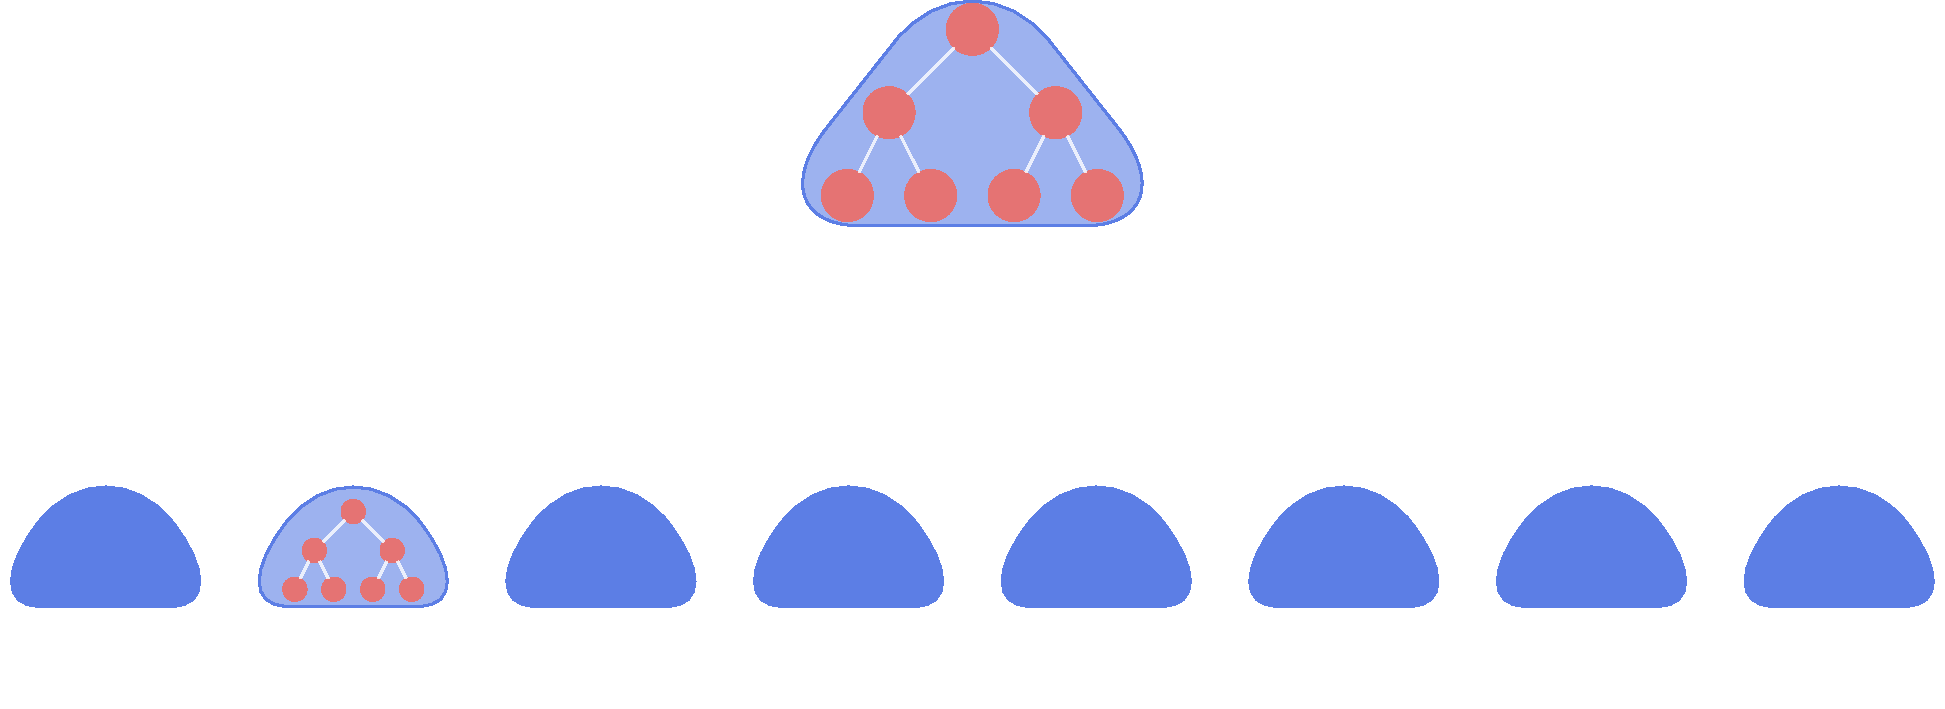
\includegraphics[width=\textwidth]{flatkdtreeExtra.pdf}
  \end{figure}
\end{frame}

\begin{frame}
  \frametitle{Flattened \kd trees}
  \framesubtitle{Advantages}

  \begin{itemize}
    \item Significantly reduced tree height
    \item More powerful look ahead to adjacent spaces when searching
    \item Greater spatial locality of tree components in memory
  \end{itemize}
\end{frame}

\begin{frame}
  \frametitle{Flattened \kd trees}
  \framesubtitle{Disadvantages}

  \begin{itemize}
    \item Additional computation per node 
      \begin{itemize}
        \item More complex path selection conditions
      \end{itemize}
    \item Greater memory footprint to fetch per node
  \end{itemize}
\end{frame}

\begin{frame}
  \frametitle{Flattened \kd trees}
  \framesubtitle{NN adjacency check}

  \begin{figure}
    \centering
    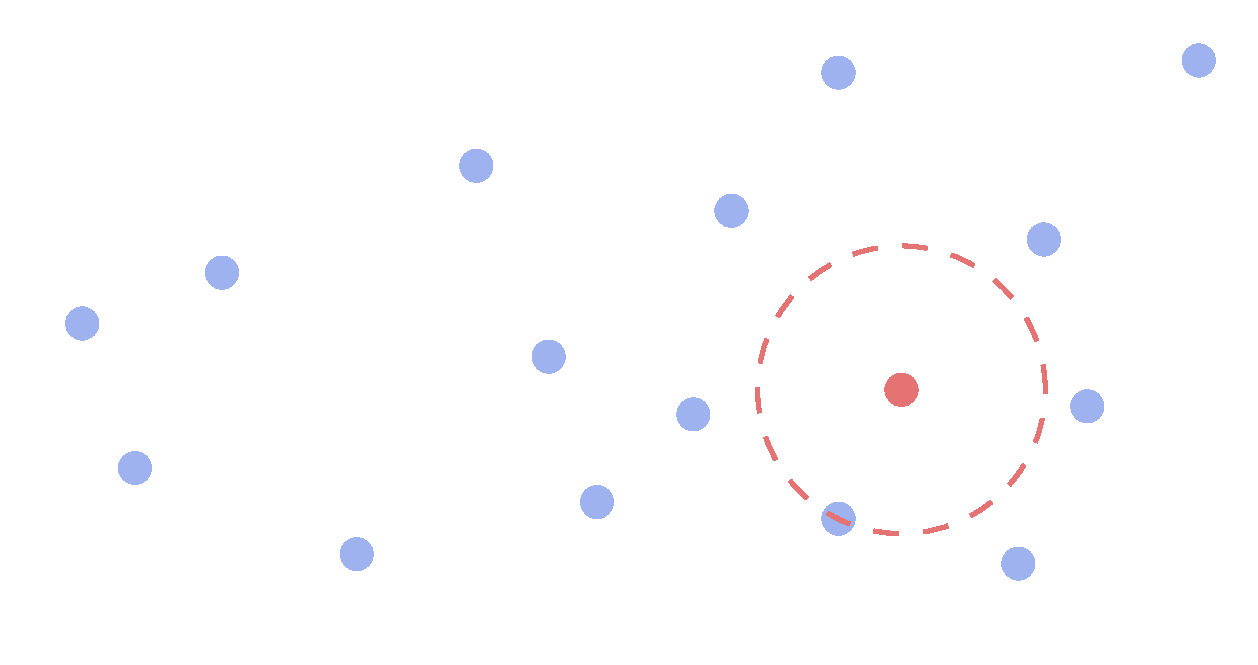
\includegraphics[width=0.85\textwidth]{nn_adjaceny_complex.pdf}
  \end{figure}

\end{frame}

\begin{frame}
  \frametitle{Flattened \kd trees}
  \framesubtitle{Initial results}

  \color{white}
  \begin{columns}[T]
    \begin{column}{0.5\textwidth}
      \vspace{-0.65cm}%
      \begin{center}
        \begin{tikzpicture}
          \centering
          \begin{axis}[
              every axis plot post/.style={/pgf/number format/fixed},
              ytick = \empty,
              ybar=-16pt,
              bar width=16pt,
              axis on top,
              height = 6.5cm,
              enlarge x limits=0.2,
              symbolic x coords ={2, 8, 16, 32, 64, 128},
              xtick={2,8,16,32,64,128},
              visualization depends on=rawy\as\rawy, % Save the unclipped values
              nodes near coords={%
                \pgfmathprintnumber{\rawy}% Print unclipped values
              },
              every node near coord/.append style={font=\DejaVu},
              y axis line style = {opacity=0},
              axis lines*=left, 
              clip=false,
              title = Pointer Dereferences,
              xlabel = Branch Factor
            ]
            \addplot[graph-red,fill=graph-red] coordinates{ (2,145) };
            \addplot[graph-blue,fill=graph-blue] coordinates {(8, 53)
              (16, 48) (32, 56) (64, 38) (128, 33)};
          \end{axis}
        \end{tikzpicture}
      \end{center}
    \end{column}
    \begin{column}{0.5\textwidth}
      \vspace{-0.72cm}%
      \begin{center}
        \begin{tikzpicture}
          \centering
          \begin{axis}[
              every axis plot post/.style={/pgf/number format/fixed},
              ytick = \empty,
              ybar=-16pt,
              bar width=16pt,
              axis on top,
              height = 6.5cm,
              enlarge x limits=0.2,
              symbolic x coords ={2, 8, 16, 32, 64, 128},
              xtick={2, 8, 16, 32, 64, 128},
              visualization depends on=rawy\as\rawy, % Save the unclipped values
              nodes near coords={%
                \pgfmathprintnumber{\rawy}% Print unclipped values
              },
              every node near coord/.append style={family=\DejaVu},
              y axis line style = {opacity=0},
              axis lines*=left, 
              clip=false,
              title = Search Time ($\mu$s),
              xlabel = Branch Factor
            ]
            \addplot[graph-red,fill=graph-red] coordinates { (2,18) };
            \addplot[graph-blue,fill=graph-blue] coordinates {(8, 36)
            (16, 42) (32, 61) (64, 66) (128, 98)};
          \end{axis}
        \end{tikzpicture}
      \end{center}
    \end{column}
  \end{columns}
\end{frame}

\begin{frame}
  \frametitle{Flattened \kd trees}
  \framesubtitle{Initial results}

  \color{white}
  {\renewcommand{\arraystretch}{1.5}
  \begin{table}
    \begin{tabular}{l r r>{\columncolor{graph-blue}} r}
      Tree & Instr. Cache Reads & Data Cache Reads & L1 Data Misses \\
      \hline \hline
      Flat \kd tree       & 77 268 111  & 31 373 726  & 314 770 \\
      %Flat \kd tree (-O2) & 21 894 724  & 5 418 211   & 343 252 \\
      Normal \kd tree     & 53 458 672  & 23 534 300  & 284 127 \\
      \hline
    \end{tabular}
    \caption{Cache usage comparison between initial flat \kd tree and nanoflann.}
  \end{table}%
  }
\end{frame}
